\documentclass[usenames,dvipsnames]{beamer}
\usetheme{Boadilla}
\usepackage{subfig} 
\usepackage{multicol}
\usepackage{color}
\usepackage[english]{babel}




\title[Clustering Approx Algs]{Local Search Approximation Algorithms for Clustering}
\author{Dave Lingenbrink, Alice Paul, Calvin Wylie}
\date{April 23, 2015}



% If you wish to uncover everything in a step-wise fashion, uncomment
% the following command: 
%\beamerdefaultoverlayspecification{<+->}


\begin{document}

\begin{frame}
\titlepage
\end{frame}


\begin{frame}
\frametitle{Motivation}
Look for structure in unlabeled data.
\begin{itemize}
\item Group plants by species
\item Find similar gene sequences to find gene families across species
\item Infer population structures
\item Crime analysis
\item PET scans to differentiate different tissues
\item Social networks and recognizing communities
\item Image segmentation and object regonition
\item Grouping customer classes and market segmentation
\end{itemize}
\end{frame}

\begin{frame}
\frametitle{$k$-Means Algorithm}
Objective: partition the data into sets $S_1, S_2, \ldots, S_k$ with means $\mu_1, \ldots, \mu_k$ to minimize $\sum_{i=1}^k \sum_{x \in S_i} ||x-\mu_i||^2$. 

\begin{center}
\includegraphics<1>[width=3.75in]{k-means-1}
\includegraphics<2>[width=3.75in]{k-means-2}
\hspace{0.6in}\includegraphics<3>[width=3in]{k-means-3}
\includegraphics<4>[width=3in]{k-means-4}
\end{center}
\end{frame}

\begin{frame}
\frametitle{$k$-Median Objective Function}
Objective: find a subset of centers $S \subseteq X$ such that $|S| \leq k$ to minimize $\sum_{x \in X} \min_{s \in S} d(x - s)$.

\begin{center}
\includegraphics<1>[width=3in]{k-median-1}
\includegraphics<2>[width=3in]{k-median-2}
\includegraphics<3>[width=3in]{k-median-3}
\includegraphics<4>[width=3in]{k-median-4}
\end{center}
\end{frame}

\begin{frame}
\frametitle{Proposed Algorithms}
\begin{enumerate}
\item Multiswap Algorithm: look at local swaps of size $p$. 
\[ \left(3+ \frac{2}{p} + \epsilon \right) \text{-approximation ratio}\]
\item Minimizing a monotone decreasing supermodular function: look at local swaps using a potential function $\psi$.
\[ \left(1 + \frac{c}{1-c} \cdot e^{-1} + \frac{1}{1-c} \cdot O(\varepsilon) \right) \text{-approximation ratio (whp)}\]
\end{enumerate}
\end{frame}

\begin{frame}
\frametitle{Hiearchical Clustering}
Look for layered structure in unlabeled data and finding a natural level of clustering.
\begin{center}
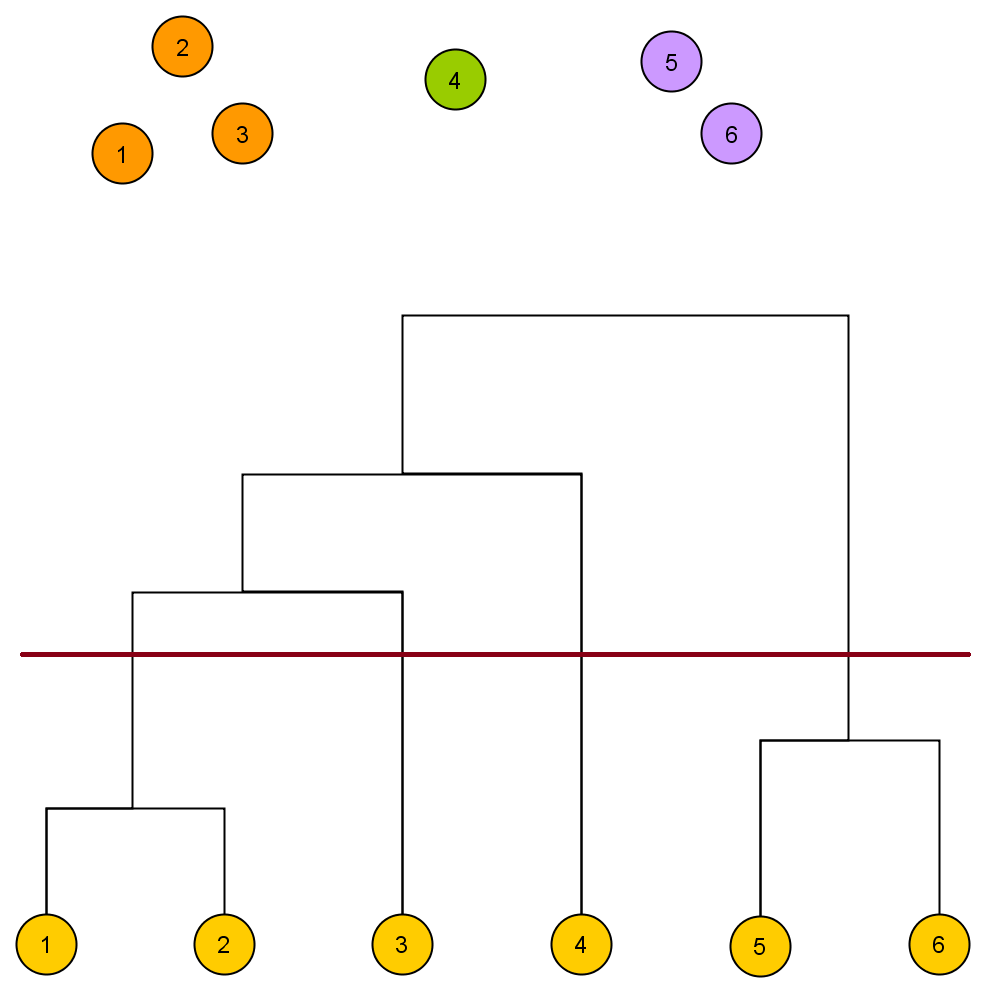
\includegraphics[width=2.7in]{hierarchical-clustering-example}
\end{center}
\end{frame}

\begin{frame}
\frametitle{Agglomerative Clustering}
Repeatedly merge the two closest clusters according to some distance function $d(C_1, C_2)$. 
\begin{center}
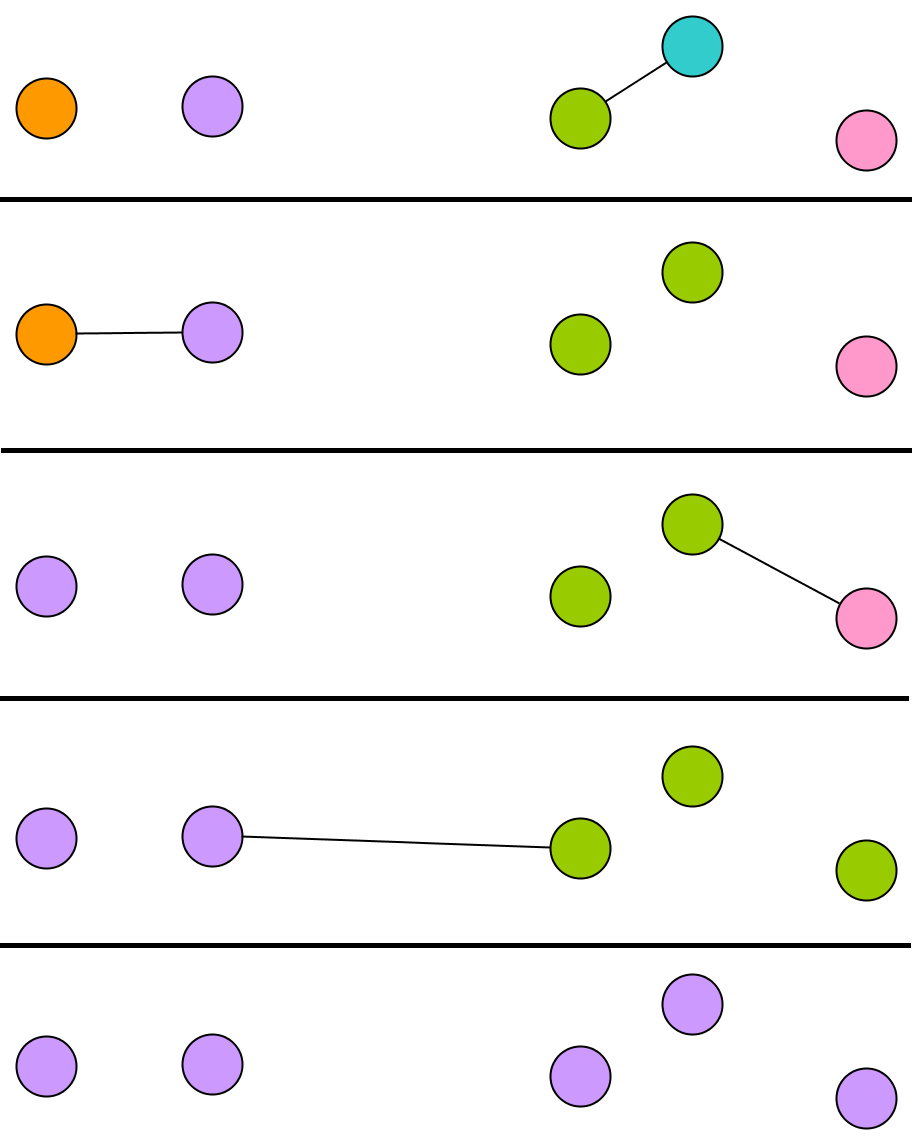
\includegraphics[width=2in]{agglomerative-clustering}
\end{center}
\end{frame}

\begin{frame}
\frametitle{Hiearchical $k$-Median Objective Function}
Find subsets $S_1, S_2, \ldots, S_n$ ($|S_i| = i$) and assignments $a_1, \ldots, a_n$ such that the clusters are nested:
\begin{enumerate}
\item $S_i \subseteq S_{i+1}$ for $i = 1, \ldots, n-1$,
\item $\forall j \in X$, if $a_{i+1}(j) \in S_i$, then $a_i(j) = a_{i+1}(j)$, and
\item $\forall j, k \in X$, if $a_{i+1}(j) = a_{i+1}(k)$, then $a_{i}(j) = a_{i}(k)$. 
\end{enumerate}

\vspace{0.5in}
There exists an approximation algorithm that given $k$-median solutions for $k=1, \ldots, n$, will generate a hierarchical clustering such that the $k$-median objective function on any level increases by at most a factor of 20.71 (or a factor of 10.03 in expectation when randomized).
\end{frame}

\begin{frame}
\frametitle{Proposed Algorithm}
\begin{center}
\includegraphics<1>[width=3in]{hierarchical-1}
\includegraphics<2>[width=3in]{hierarchical-2}
\end{center}
\end{frame}

\begin{frame}
\frametitle{Data Sets and Preliminary Results}
\begin{enumerate}
\item Iris and soybean data sets from UCI Machine Learning Repository
\item Generated Gaussian data
\item OR Library's $p$-median instances
\end{enumerate}

Comparisons in adjusted mutual information (weighted for hierarchical results), computation time, and comparison to optimal $k$-median solutions.
\end{frame}


\begin{frame}
Questions? 

\vspace{0.5in}
Learn more about the proposed algorithms:
\begin{itemize}
\item Arya et al. Local search heuristics for k-median and facility location problems. \emph{SIAM Journal on Computing}, 33(3):544-562, 2004.
\item Lin et al. A general approach for incremental approximation and hierarchical clustering. In \emph{Proceedings of the Seventeenth Annual ACM-SIAM Symposium on Discrete Algorithms}, SODA `06, pp.1147-1156, Philadelphia, PA, USA, 2006. 
\item Sviridenko, Maxim and Ward, Justin. Tight bounds for submodular and supermodular optimization with bounded curvature. arXiv:1311.4728v3 [cs.DS] 2014.
\end{itemize}
\end{frame}


\end{document}


